\section{Process Monitoring}\label{section:process-monitoring}

Here we will introduce Process monitoring console for real-time
monitoring and gathering information about currently executing processes.
The main idea behind this functionality is to:
\begin{itemize}
  \item isolate annotation process failures,
  \item improve annotation process performance,
  \item help making decisions, and
  \item improve resource management.
\end{itemize}

At the moment, GATE Teamware provides four different views in process
monitoring console:
\begin{itemize}
  \item Document Status Summary
  \item Annotation Status Details
  \item Annotator Record Summary
  \item Record Summary for All Annotators
\end{itemize}

Each view is explained in details in the following subsections.

\subsection{Document Status Summary}
To access this page, click on \emph{Process monitoring} icon in the
process list for particular project. You will see the progress of the
annotation process both in tabular and graphical
view using pie chart as shown in Figure~\ref{fig:annotationstatusoverview}.
\begin{figure}[htb]
\centering
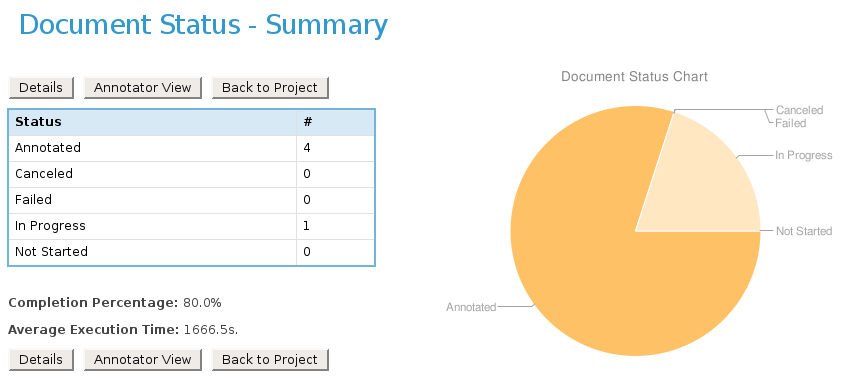
\includegraphics[scale=0.4]{annotationstatusoverview}
\caption{Document Status Summary}
\label{fig:annotationstatusoverview}
\end{figure}
The progress is displayed in real time so that it is possible
 to monitor how many documents have been finished, canceled, annotated, failed,
 in progress, and not started. When the annotation process ends, the pie chart
will disappear.

\subsection{Document Status Details}
Annotation Status Overview gives pretty condensed view about what is going on
inside process.
For more detailed view, click \emph{Details} button, and you will see the
details of the annotation project progress by document, including names of
annotators who started the work on it, finished or
 rejected the document as shown in Figure~\ref{fig:annotationstatusdetailedview}
\begin{figure}[htb]
\centering
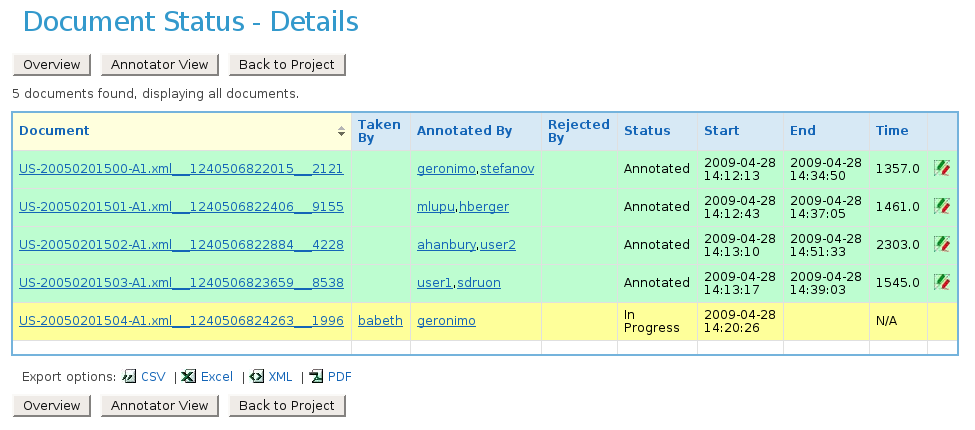
\includegraphics[scale=0.4]{annotationstatusdetailedview}
\caption{Document Status Details}
\label{fig:annotationstatusdetailedview}
\end{figure} 
 
 From this list, the status of the documents is also
 visible together with the execution time per document. For specific documents in
 the list it is possible to view details such as:
 \begin{itemize}
   \item \texttt{view (annotated) documents}, by following the document
name link. This will launch \emph{Annotation Editor}, which is described in
Section ~\ref{section:annotation-editor}
   \item \texttt{compare document annotations}; to do this follow the icon
at the end of the \emph{annotated} document row. The document with
   annotations will be loaded into the \emph{Annotation Differ} application,
which is described in Section ~\ref{section:annotation-differ}
\end{itemize}
 
\subsection{Annotator Record View}
Both annotation status views explained above are focused on the document
itself, while there might be the cases when the manager wants to see how
particular annotator performed. Therefore, we have implemented \emph{Annotator
Record View}, which you can access by clicking on the annotator name from
\emph{Document Status Details} page.
You will be able to see how many documents annotator completed, canceled,
started to annotate, along with some useful metrics. A sample \emph{Annotator
Record View} page is shown in Figure~\ref{fig:annotatorrecordview}:
\begin{figure}[ht!]
\centering
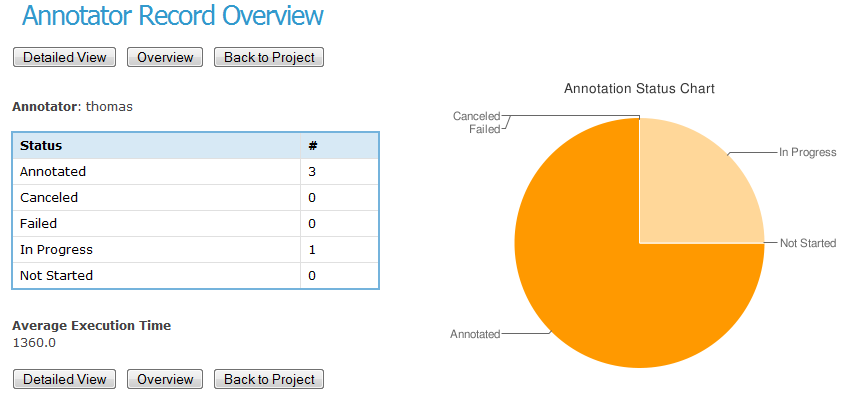
\includegraphics[scale=0.4]{annotatorrecordview}
\caption{Annotator Record View}
\label{fig:annotatorrecordview}
\end{figure}


\subsection{Record Summary for All Annotators}
In case that manager is interested to see how workload is shared among
annotators with an indicator about the average time spent per document,
\emph{Record Summary for All Annotators} screen can be very useful.
You can see this screen by clicking on \emph{Annotator View} button.
An example of this screen is shown in
Figure~\ref{fig:globalannotatorrecordview}: 
\begin{figure}[ht!]
\centering
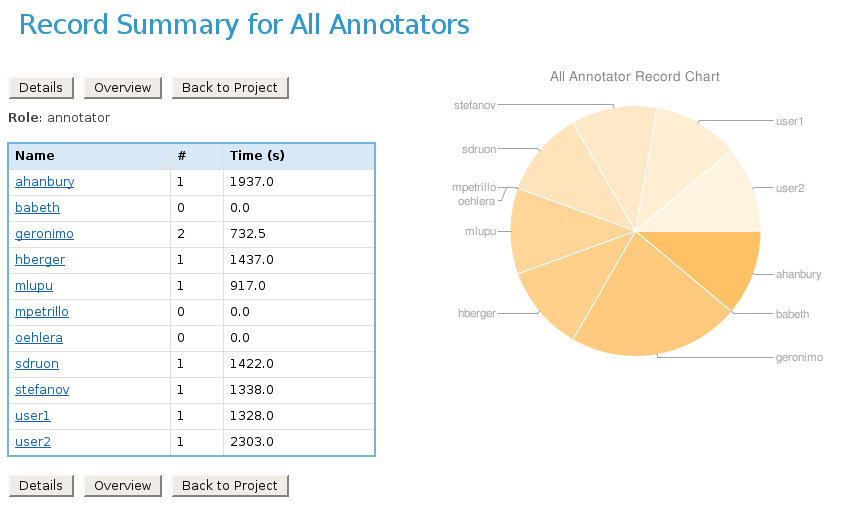
\includegraphics[scale=0.4]{globalannotatorrecordview}
\caption{Global Annotator Record View}
\label{fig:globalannotatorrecordview}
\end{figure}

